\subsection*{Synaptic Spine Calcium Dynamics}
We would like to note that the manuscript \textit{Calcium modeling of spine apparatus containing human dendritic spines demonstrates all-or-nothing communication switch between the spine head and dendrite} is currently in preparation and in this manuscript we state and explain the results described in this progress report.

The system of diffusion equations for modeling calcium dynamics given by:
\begin{align}
    \frac{\partial c_c}{\partial t} &= D_c\Delta c_c + (\kappa_b^-(b^{tot}-b)-\kappa_b^+bc_c),\\
    \frac{\partial b}{\partial t} &= D_b\Delta c_b + (\kappa_b^-(b^{tot}-b)-\kappa_b^+bc_c),\\
    \frac{\partial c_e}{\partial t} &= D_c\Delta c_e, 
\end{align}
where $c_c$ is the cytoslic calcium and $c_e$ is calcium in the ER, $(b^{tot})$ is the total concentration of CalB present in the cytosol, and $\kappa_b^+$, $\kappa_b^-$ are rate constants. We also take into account influxes at the PSD, calcium exchange mechancisms located on the ER membrane and PM, the complete set of equations is described in (cite Breit,Queisser Paper). We first established a baseline for the level of calcium concentration in the cytosol when there is no ER inside the cytosol region of the geometry. The baseline simulations were executed using the 9 spine-dendrite geometries,  Figure \ref{fig:prg1} row A, with no endoplasmic reticular (ER) and with passive ER, and a calcium influx was specified at the PSD for each spine. Both sets of basline simulations revealed that passive/absent spine apparatus organelles (the ER) have no major impact on spine-to-dendrite calcium signaling. In all cases less than 3\%  of the initial calcium concentration amplitude in the head was detectable in the dendrite. When the ER was added as a passive compartment (i.e., when it was present as a geometric obstacle, but without any calcium exchange mechanisms), similar and near-zero dendritic calcium concentration profiles are observed in the respective spines Figure \ref{fig:prg1} row B. Therefore, calcium influx at the PSD alone without intracellular calcium dynamics from the ER is not enough to induce spine-to-dendrite calcium coupling; in particular, only a small fraction of released $\textrm{Ca}^{2+}$ ions reaches the dendritic compartment. However, with active ER there exists a critical RyR density where by we have significan calcium signaling in the dendritic region Figure \ref{fig:prg1} row C.

\begin{figure}[h]
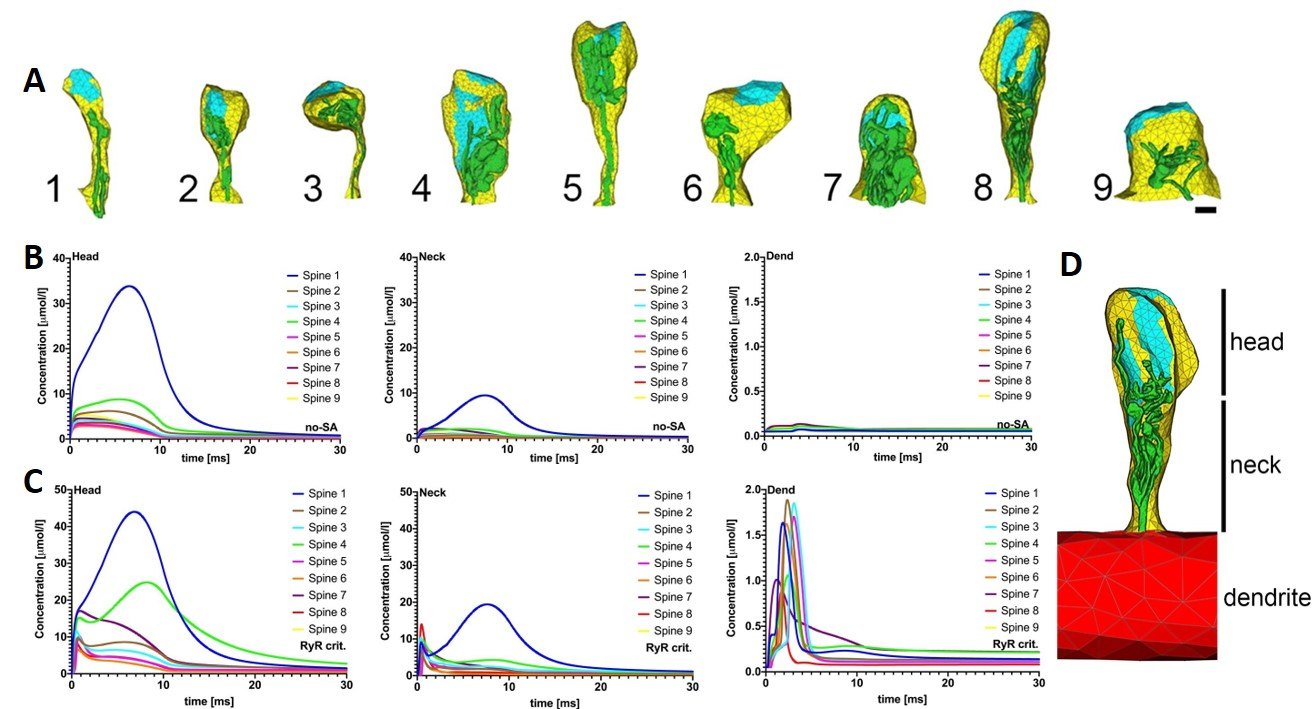
\includegraphics[width=\linewidth]{inc/img/Picture1.jpg}
\caption{}
\label{fig:prg1}
\end{figure}

We determined that when the ER is active with RyRs and SERCA pumps there is a critical RyR density $\rho_{RyRcrit}$, Figure \ref{fig:prg2}A such that if $\rho_{RyR}<\rho_{RyRcrit}$ then there is no spine-dendrite calcium signaling and if $\rho_{RyR}\geq\rho_{RyRcrit}$ there is spine-to-dendrite calcium signaling (Include a picture showing this). This was carried out by running a sequence of simulations where the RyR density parameters was increased  starting from 0.00 $\mu m^{-2}$ to 5.00 $\mu m^{-2}$ at increments of 0.01 $\mu m^{-2}$. We tested whether changes in $\textrm{Ca}^{2+}$ entry at the synapse affect the critical RyR density by successively increasing the $\textrm{Ca}^{2+}$ flux density at the PSD, and the simulations demonstrate that calcium coupling occurs at the same RyR density, regardless of the initial $\textrm{Ca}^{2+}$ influx Figure \ref{fig:prg2}B. Therefore, ryanodine receptors of spine apparatus control spine-to-dendrite $\textrm{Ca}^{2+}$ signaling. We also carried out simulations by which we varied the neck diameter of the spine morphologies, and we determined that critical RyR density was affected by changes in the spine neck diameter. 

We are currently running simulations incorporating voltage dependent calcium channels (VDCCs) to determine under what conditions we have string spine-to-dendrite calcium signalling and calcium wave propagation through the dendrite. Current simulation results demonstrate that having either PSD calcium influx or VDCC  release is sufficient for calcium signaling to the dendrite; however, having each alone is not enough to produce stable calcium wave propagation.
\begin{figure}[h!]
\centering
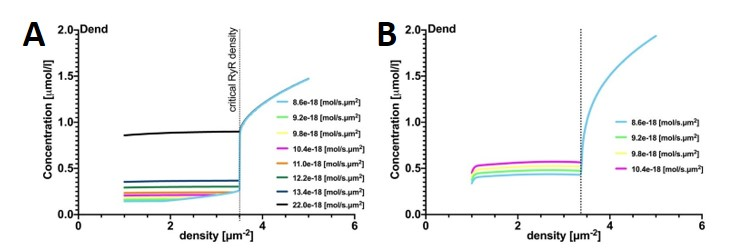
\includegraphics[width=0.65\linewidth]{inc/img/Picture2.jpg}
\caption{}
\label{fig:prg2}
\end{figure}



% We systematically tested whether changes in spine neck diameter can affect spine-to-dendrite Ca2+ communication. To address the role of spine neck %plasticity in spine-to-dendrite Ca2+ signalling we ran simulations by using the reconstruction of one of our spines and manually widened the spine neck %by 10\%, 20\%, and 40\%, while keeping the RyR density and the SA morphology constant. While the Ca2+ dynamics in the spine head remain unchanged, we %observed that increasing the spine neck width caused a decrease in peak Ca2+ near the spine apparatus (SA) membrane, therefore producing insufficient %Ca2+ release from the SA store to maintain spine-to-dendrite coupling. We then tested whether an increase in RyR density could balance morphology %plasticity in order to maintain coupling even under spine growth and reorganization. For each of the modified spines we incrementally increased the RyR %density and observed that a critical RyR density can be determined for all spines. Naturally, this critical value increases with increasing neck width; %therefore, the critical RyR density depends on spine morphology.
 
%Next we execute Calcium Pulse runs for at least 3 seconds simulation time to observe the coupling effects between the spine region of the neuron and %the dendrite region of the neuron for a fixed RyR density and different calcium influx pulse frequencies. These particular simulations were performed %with supercritical RyR density, each at 1 Hz, 3 Hz, 5 Hz, 10 Hz, and 20 Hz frequencies. We observed that for particular spines, there were particular %ranges of frequencies where by we observed spine-to-dendrite calcium coupling, we hypothesize this is attributed to the calcium release and %sequestration cycle due to SERCA pumps. 

\subsection{Whole Cell Dynamics Progress}
For the proposed sub-project \textbf{Whole Cell Dynamics}
